\documentclass[12pt,a4paper]{article}

% Packages
\usepackage[utf8]{inputenc}
\usepackage{amsmath,amssymb}
\usepackage{graphicx}
\usepackage{geometry}
\usepackage{tikz}
\usepackage{enumitem}
\geometry{margin=1in}
\setlist{nosep}

% Title
\title{\textbf{Color Science \& Video Editing Notes}}
\author{}
\date{}

\begin{document}
\maketitle

\section{Colorspace Transforms}
\begin{itemize}
    \item \textbf{Definition}: A method to convert image or video data from one color space and gamma curve to another.
    \item \textbf{Steps in DaVinci Resolve}:
    \begin{enumerate}
        \item Set \textbf{Input Color Space \& Gamma} in CST (Color Space Transform) node to match the camera’s format.
        \item Set \textbf{Output Color Space \& Gamma} to:
        \begin{itemize}
            \item DaVinci Wide Gamut
            \item DaVinci Intermediate
        \end{itemize}
        \item Perform editing and color grading in the wide gamut space.
        \item Add a CST Out Node to convert back to \textbf{Rec.709, Gamma 2.4} for delivery.
    \end{enumerate}
    \item \textbf{Notes}:
    \begin{itemize}
        \item Clipping occurs when color values go outside the gamut.
        \item Images may lose bright or saturated colors if not transformed correctly.
    \end{itemize}
\end{itemize}

\section{Key Concepts}

\subsection{Gamma}
\begin{itemize}
    \item Non-linear distribution of luminance values.
    \item Used for:
    \begin{itemize}
        \item Gamma correction (to compensate for display response).
        \item Monitor calibration.
    \end{itemize}
    \item Equation:
    \[
    V_{out} = A \cdot (V_{in})^{\gamma}
    \]
\end{itemize}

\begin{center}
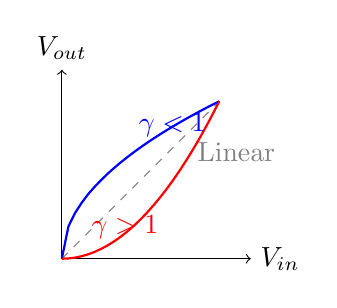
\begin{tikzpicture}[scale=2]
    % axes
    \draw[->] (0,0) -- (1.2,0) node[right] {$V_{in}$};
    \draw[->] (0,0) -- (0,1.2) node[above] {$V_{out}$};
    % linear line
    \draw[dashed, gray] (0,0) -- (1,1) node[pos=0.8, below right] {Linear};
    % gamma curves
    \draw[blue, thick] plot[domain=0:1] (\x, {\x^(0.5)});
    \draw[red, thick] plot[domain=0:1] (\x, {\x^(2)});
    % labels
    \node[blue] at (0.7,0.85) {$\gamma<1$};
    \node[red] at (0.4,0.2) {$\gamma>1$};
\end{tikzpicture}

\textit{Gamma Curves: effect of different $\gamma$ values}
\end{center}

\subsection{Dynamic Range}
\begin{itemize}
    \item Measured in \textbf{stops (f-stops)}.
    \item $1$ stop = doubling or halving of light.
    \item Formula:
    \[
    f\text{-stop} \propto \frac{1}{\text{aperture}}
    \]
    \item More stops $\Rightarrow$ more details in shadows and highlights.
\end{itemize}

\subsection{Gamut}
\begin{itemize}
    \item Defines the complete range of colors that can be represented in a given color space.
\end{itemize}

\begin{center}
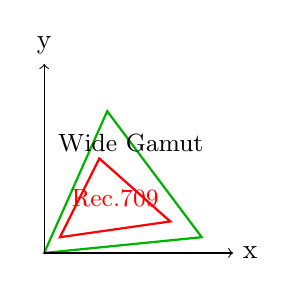
\begin{tikzpicture}[scale=2]
    % triangle approximation of gamut
    \draw[thick, green!70!black] (0,0) -- (1,0.1) -- (0.4,0.9) -- cycle;
    % Rec.709 inside
    \draw[thick, red] (0.1,0.1) -- (0.8,0.2) -- (0.35,0.6) -- cycle;
    % labels
    \node at (0.55,0.7) {\small Wide Gamut};
    \node[red] at (0.45,0.35) {\small Rec.709};
    % axes
    \draw[->] (0,0) -- (1.2,0) node[right] {x};
    \draw[->] (0,0) -- (0,1.2) node[above] {y};
\end{tikzpicture}

\textit{Color Gamuts: Rec.709 vs. Wide Gamut (CIE xy diagram simplified)}
\end{center}

\section{Color Models}
\begin{itemize}
    \item \textbf{RGB}: Basis for most display devices.
    \item \textbf{CIE 1931 XYZ}: Mathematical standard for defining colors.
    \item \textbf{HSV (Hue, Saturation, Value)} and \textbf{HSL (Hue, Saturation, Lightness)}:
    \begin{itemize}
        \item Hue: Type of color (red, green, etc.)
        \item Saturation: Strength or intensity of color.
        \item Value/Lightness: Brightness.
    \end{itemize}
\end{itemize}

\begin{center}
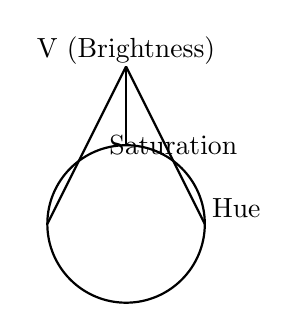
\begin{tikzpicture}[scale=2]
    % cone shape for HSV
    \draw[thick] (0,0) circle (0.5);
    \draw[thick] (0,1) -- (-0.5,0) (0,1) -- (0.5,0);
    \draw[thick] (0,1) -- (0,0.5);
    \node at (0,1.1) {V (Brightness)};
    \node at (0.7,0.1) {Hue};
    \node at (0.3,0.5) {Saturation};
\end{tikzpicture}

\textit{HSV Color Model (conceptual cone)}
\end{center}

\section{Video Production Hardware (Blackmagic Design)}
\begin{itemize}
    \item SDI Routers
    \item Cintel (Film scanner)
    \item Ultimatte (Compositing tool)
    \item ATEM Switchers
    \item Desktop solutions
    \item Streaming devices
    \item Disk Recorders
    \item Cameras
    \item RAW format
\end{itemize}

\textit{Note: These are not video editing software, but hardware tools used in production pipelines.}

\section{Extra Notes}
\begin{itemize}
    \item Colors outside gamut appear clipped or inaccurate.
    \item Rec.709 is the standard for HD broadcast.
    \item DaVinci Wide Gamut preserves more color detail for grading.
    \item Log profiles (C-Log, S-Log, V-Log) are used to capture wide dynamic range and require LUTs or CST for proper viewing.
\end{itemize}

\end{document}